	\documentclass{llncs}
		\usepackage{llncsdoc}
		\usepackage[noend]{algpseudocode}
		\usepackage{subcaption}
		\usepackage{subfig} 
		\usepackage{graphicx}
		\usepackage{usual}
		\usepackage[rflt]{floatflt}
		\usepackage{amsmath}
		\usepackage{eulervm}
		\usepackage{fontenc}
		\usepackage{mathrsfs}
		\usepackage{multirow}
		\usepackage{array}
		\usepackage[rflt]{floatflt}
		\usepackage{makecell}	
		\usepackage{xcolor, soul}
		\sethlcolor{yellow}	
		
		\begin{document}
				\title{\vskip -10pt Dominance in dialogue of cooperative negotiation}
				\maketitle
			\section{Introduction}
			Dialogue systems are artificial systems capable to hold a conversation with a human user, usually to achieve certain objective or fulfill a task.
			% Existing conversational agents provided with dialogue system play different roles like 
			
			During a human-human dialogue, interlocutors establish a social relationship that affect their behaviors. Previous researches have shown that people tend to respond to computers as social actor [bickmore], which lead the community to assess the psychosocial relationship between the person and the agent during their interaction. 
			A growing body of research is investigating the use of appropriate social behavior for virtual agents in different roles and types of user-computer relationship.
			For example, Bickmore studied the impact of trust ...[To complete]
			
			
			In this paper, we are interested in modeling a dialogue system for social dialogue in which user and agent cooperate in order to achieve a common objective.  We believe that individuals that collaborate to fulfill an objective (for example: find a restaurant for dinner), have their own preferences in the way to do it, which lead them to conduct a \emph{cooperative negotiation} about their preferences in order to determine a trade-off that satisfy both interlocutors. Moreover, scholars in social psychology and communication investigated the impact interactive effects of relations and emotion in negotiation, and proved that  \emph{interpersonal dominance} affect the strategies of negotiators. Our objective is to build an agent that can perceive the established relation of dominance and adapt its strategy of negotiation to the relation. 
			
			In the next section, we review related works on designing social agents. Section 3 will relate our definition of dominance based on research on social psychology. In section 4, we present our model of dialogue. Section 5 will discuss our experiment and the analysis obtained results. 
			
			\section{Related works}
			
			
			\section{Dominance in dialogue}
			\par Despite the various definitions of dominance available in the fields of interpersonal communication and psychology, scholars are converging to a general definition of dominance as the power to produce intended effects, and the ability to influence the behavior of other person in the conversation. (Bachrach \& Lawler, 1981; Berger, 1994; Burgoon et al.,
			1998; Foa\& Foa, 1974; French \& Raven, 1959; Gray-Little \& Burks, 1983;
			Henley, 1995; Olson \& Cromwell, 1975; Rollins \& Bahr, 1976). Dominance is generally viewed as a personality trait, or to describe the social role of an individual inside a group. However, in the context of communication, dominance is a dyadic variable where one individual's attempt of control is necessarily acquainted by the partner in the interaction.(Rogers-Millar and Millar, 1979,Dunba and Burgoon, 2005). 
			\par Dominant behaviors in a conversation can contribute either positively or negatively to the discussion. For example, positive contributions include actions such as keeping the conversation going, orient the task decision, by making quick decisions and conclusions etc. Negative contribution may include not considering the partner in the conversation, for example, not giving the occasion to express his opinion, not open to criticism. In addition, expressing verbally the dominance can be viewed as offensive and unjustified (K,Zablotskaya). Giving these contributions to the conversation, several researches get interested to detect  behaviors related to the dominance during the conversation. We focus essentially on the context of conversation of negotiation, where several researches already proved the impact of dominance on the negotiation(VAN KLEEF, 2005)
			
			\subsection{Behaviors of dominance in dialogue}
			Several scholars studied behaviors related to the dominance in order to gain a better understanding to social relations. During a conversation, dominance can be perceived through verbal and nonverbal behaviors. We present in this section behaviors related to dominance that can be perceived in a conversation of cooperative negotiation.
			\subsubsection{Non-verbal behaviors:}
			At the non-verbal level, a wide range of behaviors have been associated with dominance. (Dunbar \& Burgoon) divide non-verbal behaviors into classes such (kinesics, vocalic, ). First, kinesics behaviors are considered as the richest of all the codes that includes facial expression, body movements, gestures. Indeed, dominant individuals are related with high visual ratio (high looking while speaking / listening)(burgoon).  Furthermore, (Dunbar, Burgoon 2005) found that the more body control an individual had the more observers perceived her as dominant. In addition, dominant individual are more susceptible to use gesture when they talk.  
			\par  Second, voice cues of dominance manifest by speaking duration, speaking intensity, voice control and pitch. Dominant individuals speak loudly and more frequently and might cause interruption while other are talking (Dunbar, Burgoon 2005).
			
			\subsubsection{Verbal behaviors:}
			verbal behavior of dominance in the dialogue is related to the type of \textit{strategies} that individuals choose in order to take control of the other especially during a negotiation. Therefore, dominant negotiators tend to end up with the larger share of the pie (Giebels, De Dreu, \& Van de Vliert, 2000). 
			\par A considerable body of research has documented the effects of dominance on negotiation behaviors and outcomes. First, dominant negotiator have higher aspirations, demands more and concede less(De Dreu, 1995). Second, dominant negotiator control the flow of the negotiation. Indeed, dominant behavior increase task orientation and goal-directed behaviour (Galinsky,Gruenfeld, \& Magee, 2003). Finally, dominant negotiator tend to not pay attention to less dominant negotiators Fiske (1993). The idea is that high-dominant individuals have many resources and can often act at will without serious consequences, while submissive individuals, have to be more careful because they are more dependent on other people. In addition, they are motivated to gain or regain control over their outcomes by paying close attention to the people on whom they depend.
			
			\par We are interested in this paper to the verbal behaviors for two main reasons. First, verbal behaviors are directly related to \emph{the strategies} deployed during the negotiation. In addition our dialogue system is text oriented, which make the non-verbal behavior impossible to reflect during the dialogue. 
			We present in the next section the decision model based on dominance behaviors. 
			
			\subsection{Principles of dominance in negotiation}
			
			\section{Model of negotiation based on dominance}
	%		
	%			 \subsection{Model of preferences}
	%			  \subsection{Model of communication}
	%			  \subsection{Strategies of negotiation (decision)}
		\subsection{Domain model}
		Consider a sequence of criterion sets $C_1, C_2, ..., C_n$ and an options set defined as the cross-product:
		$O = C_1 \times C_2 \times \ldots C_n$.
		
		For example, for restaurants, the criteria might be: \\
		Cuisine = \{Chinese, French, ...\} \\
		Cost = \{cheap, expensive, ...\} \\
		Atmosphere = \{quiet, lively, ...\} \\
		
		\par and a restaurant options might be: 
		\begin{itemize}
			\item $[Chinese, cheap, lively]$. 
			\item $[Chinese, expensive, quit]$.   
			\item $[Chinese, expensive, lively]$.
			\item $[French, cheap, quit]$.  
			\item $[French, expensive, quit]$.   
			\item $[Chinese, expensive, lively]\ldots$ 
		\end{itemize}
		
		
		\subsection{Self model} 
		
		\subsubsection{Preferences for self}
		Preferences are partial orders (transitive, asymmetric binary relations) on the criterion sets. The preference relation on the criterion set $C_i$ is denoted by $\prec_i$.
		
		Let $\prec$ denotes the sequence of preferences $\{ \prec_i, \prec_2, ..., \prec_n\}$
		
		\subsubsection{Self satisfaction function} 
		
		Satisfaction is a function normalized to [0,1] that evaluates an element of a criterion set relative to the corresponding preference relation, defined as follows.
		
		For $c \in C_i$ and $\prec_i$:
		
		$$sat(c, \prec_i) =	1 - \left( \frac{|\{d : d \neq c \  \wedge \ (c \prec_i d)\}| }{( |C_i| - 1 )}\right)  $$
		
		Satisfaction is generalized to options as a weighted sum.
		For $o \in O$ and where $o_i$ is the i-th element of $o$ and $\prec_i$ the i-th element of $\prec$.
		
		$$sat(o, \prec) = \frac{\sum_{i}^{n} sat(o_i, \prec_i) }{n} $$
		
		
		\subsection{Dialogue model}
		We present in the section the knowledge that the agent gather and processed from the dialogue.
		
		\subsubsection{Other model}
		We do not have detailed knowledge of the preferences of the other; the agent only knows which criteria values the other has said are acceptable or unacceptable.
		
		Let the collection of $A_i \subseteq C_i$ be the criterion values that are acceptable to the other, and $U_i \subseteq C_i$ be the criteria values that are unacceptable.  We assume $A_i \cap U_i = \emptyset$.  Note	that some values are thus unknown.
		
		Then the acceptability of a criterion $c \in C_i$ is a function normalized to [0,1] and defined as follows.
		$$ other(c, A_i, U_i)= \left\{\begin{array}{ll}
		1	 & \mathrm{if\ }  c \in A_i\\
		0    & \mathrm{if\ }c \in U_i\\
		0.5	 & \mathrm{otherwise}
		\end{array}\right.$$
		This function is generalized to options as a weighted sum.
		
		$$other(o, A, U) = \frac{ \sum_{i}^{n} other(o_i, A_i, U_i) } {n}$$ 
		
		\subsubsection{Negotiation state}
		During a negotiation, negotiators express two types of utterances: %that we name \emph{statement moves} and \emph{negotiation moves}. 
		
		\begin{itemize}
			\item \emph{Statement move:} Speaker share information about its preferences (StatePreference) or ask other about his preferences (askPreferences).
			\item \emph{Negotiation move:} Interlocutors negotiate about the different options of a topic (Propose, accept or reject proposals).
		\end{itemize}
		
		
		In order to produce coherent dialogues, the agent keeps track about the different states of the dialogue, that each move updates. 
		
		The negotiation might focus on each criterion of the discussed topic. For example, in a negotiation on restaurants, speakers might negotiate about the type of \textit{cuisine}, and the \textit{ambiance} to choose.  We note $D$ the set of criteria which have been discussed during the dialogue. When speakers agree on a value of a criterion to choose, the negotiation on this criterion is considered as \textit{closed}. We note $Cl$ the set of closed criteria.
		
		For each discussed criterion $C_i \in D$, the agent register the following information:		
		\begin{itemize}
			\item Let the collection of $S_i \subset C_i$ be the criterion values stated by the agent in the dialogue.
			\item Proposals which are made during the negotiation by both negotiators might have different status. They can either be accepted or rejected with respect of the decisional model (See section \ref{decision}).
			\subitem - $P_i$ is the set of  values which have been proposed in the negotiation.
			\subitem - $T_i$  is the set of values which have been accepted in the negotiation.
			\subitem - $R_i$  is the set of values which have been rejected in the negotiation.
		\end{itemize}
		
		Moreover, interlocutors are allowed to make proposals of options. Therefore we define the same structure of proposals for the options; $P, R, T$
		
		\subsection{Decision based on dominance in negotiation}
		\label{decision}
		\subsubsection {Dominance and concession}
		Let  $dom \in [0, 1] $ denotes the dominance of an agent (self) in the relationship.  It is a constant for a given agent in a given relationship.
		
		The weight that an agent gives to its self-satisfaction relative to	the satisfaction of the other is a time-varying function normalized to 	[0,1] of its dominance, defined as below.
		$$self(dom, t) = \left\{\begin{array}{ll}
		dom & \mathrm{if\ } (t \leq \tau)\\
		max(0, dom - (\frac{\delta}{dom} . (t - \tau))) & \mathrm{otherwise}
		\end{array}\right.$$
		
		
		where is $t \geq 0$ is the number of open or rejected proposals.
		
		This is called the "concession curve", where $\tau > 0$ and $\delta > 0$
		are parameters of the theory in general and are initially assumed to
		be 2 and 0.1, respectively.
		
		Therefore, the acceptability of a value $c \in C$  is relative to the weight an agent gives to its self satisfaction:
		
		$$acc(c, t) = sat(c, \prec_i) \geq  \beta \times Self(t)$$
		with $\beta > 0 $.
		
		This function is generalized to options:
		$$acc(o, t) = sat(o, \prec) \geq  \beta \times Self(t)$$
		
		
		\subsection{Lead of the negotiation}
		
		
		\subsubsection{Choosing an utterance type}
		Let $V$ be the set of available options (values), such that option :$ V\rightarrow O$	i.e., each value is a "name" for an option.  For example, V is the set of restaurants that are mutually known to the participants. This can be a many-to-one function, e.g., there could be two restaurants with same criteria.		
		
		We present in the following the possible responses and their applicability conditions. Note that each line (utterance)  assumes that the previous ones are already not applicable.
		
		$ chooseUtterance(dom, t, V, \prec, A, U) = $ \\
		
		
		\textbf{if(\textbf{dom  $>\sigma$})} 
		\begin{table}
		\centering
	
		\begin{tabular}{|p{3cm}|p{9cm}|}
			\hline
			\textbf{Utterance type} & Condition \\
			\hline
			Negotiation success & $\exists o \in T$   \emph{OR} $o \in P$ such that  $acc(o,t) = true$ \\
			\hline
			Negotiation failure & $ \forall o \in O$,  $o \in O$  \emph{OR} $acc(o,t) = false$\\
			\hline
			State & $type(u^{-1}) = AskPreference$  \textit{ and }
			$n < \alpha$ (with $n$ the number of successive statement moves)\\
			\hline
			AcceptPropose & $\exists c \in P_i$ / $acc(c,t)= true$ \\
			\hline
			RejectPropose & $\exists c \in P_i$ / $acc(c,t)= false$ \\
			\hline
			Propose & Otherwise  \\
			
			\hline
		\end{tabular}
		\end{table}

		
		\textbf{if(\textbf{dom  $ \leq \sigma$})} 
		\begin{table}
			\centering
		\begin{tabular}{|p{3cm}|p{9cm}|}
			\hline
			\textbf{Utterance type} & Condition \\
			\hline
			Negotiation success &  $\exists o \in T$ \\
			\hline
			Accept & $\exists c \in P_i$, $acc(c, t)=true $ \newline \emph{OR}   \newline $ \exists o \in P$ ,  $acc(o, t) =true$ \\
			\hline
			RejectState & $ [\exists c \in P_i$, $acc(c, t)= false $  \emph{OR}   $ \exists o \in P$ ,  $acc(o, t)=false]$ \newline  \emph{AND} $t<\tau$.\\
			\hline
			Propose & $\exists c$ / $other(c, A_i, U_i)  = 1 $  \emph{and}
			\newline $acc(c, t)=true$
			\newline \emph{OR}  
			\newline $\forall c \in C_i$,  $c \in T_i$\\
			\hline
			Ask &  \textbf{(}$t> \tau,$ \emph{and} 
			$\exists c \in P_i /$
			$ acc(c, t)=false$\textbf{) }
			\newline \emph{OR}
			\newline $ \forall c \in C_i,other(c, A_i, U_i)=0.5$ \\
			\hline
			
			State & $type(u^{-1}) = AskPreference$
			\newline \emph{OR}
			\newline $\exists x,other(x, A_i, U_i) \not = 0.5 $ 
			\newline \emph{OR}
			\newline $ \exists C \in \mathcal{C}, A_i(C) = Unkown$
			\\
			\hline
			Propose & Otherwise \\
			\hline
		\end{tabular}
			\end{table}
		
		\subsubsection{Choosing a value for an utterance} 
		
		
		Let be $\{V' \subset V$ / $\forall v \in V'$ $ acc(v,t) = true\}$ be the list of agent's acceptable values. 
		
		The value for a proposal should be tolerable for both interlocutors. Therefore,  in addition to self preferences, the agent should considers other preferences. 
		
		We define a tolerance function of a criterion $c \in C_i$ as a function normalized to [0,1] and defined as below.
		
		$$tolerable(dom, t, c, \prec, A, U) = self(dom, t) . sat(c, \prec_i) \ +\  (1 - self(dom, t)) . other(c, A_i, U_i)$$
		
		Tolerance is generalized to options as a weighted sum.
		
		$$tolerable(dom, t, o, \prec, A, U) = \frac{ \sum_{i}^{n} tolerable(dom, t, o_i, \prec_i, A_i, U_i) } {n}$$ 
		
		
		
		The following function returns the most tolerable element of $V'$ to make a proposal.
		
		$$ chooseValue(dom, t, V, \prec, A, U) =	\operatorname*{arg\,max}_{name \in V} tolerable(dom, t, option(name), \prec, A, U) $$
		
		Note that argmax may not be unique.  The following function returns the most tolerable element of	criterion $C_i$.
		
		$$chooseCriterion(dom, t, V, \prec, A, U, C_i) = option(chooseValue(dom, t, V, \prec, A, U, C_i))_i$$
		
		
		
		
		\subsection{Summary of general parameters }
		\begin{itemize}
			
			\item $\sigma \in $[0,1] : boundary between submissive and dominant used in
			choosing an utterance type
			%		\item $\beta$:  a value that represent the minimum score that a value has to get to be positively satisfiable to the agent preferences in the negotiation. Note that $\beta = const \times self(dom,t)$.
			\item $\tau > 0$ : the minimum number of open or rejected proposals before.
			concession begins
			\item $\delta > 0$ : parameter in slope of concession curve.
			\item $u^{-1}$ refers to the previous utterance.
			\item $\alpha> 0$: the maximum number of successive statement moves.
			
			
		\end{itemize}
		
	
				  
		\section{Evaluation}
		
		 We built a conversational agent able to deploy a strategy of negotiation based on its perception of interpersonal relationship of dominance. 
		 
		 
		 In order to validate our model, we present in this section a perceptual experiment in which participants have to determine the behaviors of two agents generated using our model. 
		 
			\subsection{Study design}
		We developed an experimental scenario in which we generate dialogues of negotiation between two agents implemented with the proposed model. We used a simple topic of "negotiation about a restaurant where to have dinner".
		
		We manipulated two parameters in the generation of dialogues. First, the initial value of dominance \textbf{dom} (see section \ref{decision}). The purpose was to define the behavior of agents in negotiation. 
		We aimed to make the first agent adopt more a dominant behavior by initiating the value of its dominance \textbf{dom} in the higher range (dom  $>\sigma$). Complementarity, the second agent had to adopt a submissive behavior. Therefore we initiated its \textbf{dom} to be in the lower range. (dom  $ \leq \sigma$)
		
		The second manipulation involved varying the initial preferences of both agents.  We manipulated the initial preferences to be either similar or different. We used the metric of Kendall distance \cite{bra2013Kendall} in order to compute the distance between two preferences sets (see section \ref{decision}).  
	%	\begin{table} 
	%		\centering
	%		\begin{tabular}{|c|c|}
	%			\hline
	%			Models & Distance \\
	%			\hline
	%			(Model1, Model2) & 0.98\\
	%			(Model2, Model3) & 0.90 \\
	%			\hline
	%		\end{tabular}
	%		\caption{Kendall distance between the models of preferences}
	%	\end{table}
				
		\subsection{Hypotheses}
		 We investigated three main hypotheses about the perception of agents behaviors of dominance during the negotiation. 
		 \begin{itemize}
		 	\item  \textbf{H1:} The more an agent is dominant the more he is perceived as individualist and self-centred.  
		 	
		 	\item \textbf{H2:} Agents with lower dominance will make larger concessions.
		 	
		 	\item \textbf{H3:} Agents with lower dominance are perceived as having a lower level of demand comparing to agents with higher dominance. 
		 	
		 	\item \textbf{H4:} Agents with higher dominance are more likely to take the lead of the negotiation. In addition they are perceived to adopt a goal-directed behavior. 
		 	
		 	\item \textbf{H5:} In the condition where initial preference sets of agents are similar, the behaviors of dominance will not be visible, because the negotiation converge quickly.
		 	
		 \end{itemize}
				
		\subsection{Experimental Procedure}
		
		We conducted a between-subject study using an online crowdsoursing website \emph{CrowdFlower} \footnote{https://www.crowdflower.com/}. 
		Each generated dialogue had a questionnaire. There were 12 questions (including 2 test questions).
		
		Participants had to judge each agent behaviors in the proposed dialogues. Agents were described as two friends trying to find a restaurant where to have dinner. We wanted to avoid skewing the participant's perception by the fact that negotiators are artificial agents. Participants were invited to read the assigned dialogue and answer the corresponding questionnaire. 
		
		\subsection{Participants}
		A total of 10 subjects participated to the experiment. They were recruited through the website \emph{Crowdflower.com}, for which each subject received \textit{20 cents} for the task. 
		
		
		We limited the participant pools to native English speakers. Test questions were included to check the sanity of the answers. We eliminated participants providing wrong answers to our sanity questions. The final number of participants were 10. 
		
		\subsection{Results}
		\hl{We should add in the begging a study about the relation between questions for the same principle $\alpha$ crombach}
		
		
		\par We used the T-Student analysis to analyze the obtained results for the different conditions. 
		
		
		Our first hypothesis (H1) predicted that participants perceive agents with lower dominance  to care more for other preferences than agents with higher dominance would do. Our analysis confirmed our prediction; participants rated agents with lower dominance to consider the preferences of other (M=3.8, SD = 0.79), than they did with agents having higher dominance (M=2.2, SD=1.14), \emph{p =.011} (see Figure \ref{considerOther}).
					\begin{figure}[h]
						\centering
						\caption{\label{considerOther} The results for the  hypothesis H1}
						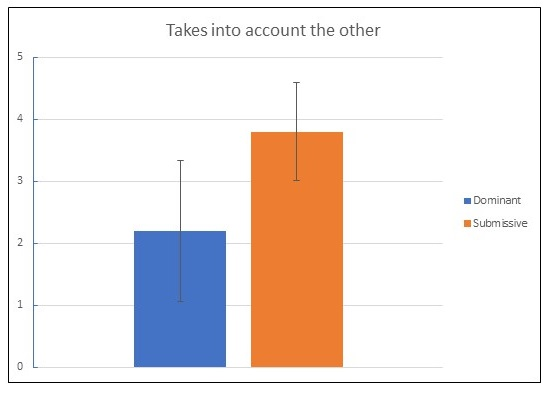
\includegraphics[width=3in]{plots/considerOther}
					\end{figure}
		
		\par Our second hypothesis (H2) predicted that agents with lower dominance will be perceived to make larger concessions. Participants reported that agents with lower dominance  make larger concessions in the negotiation, (M=3.4, SD=1.07), than agents with higher dominance(M=2.6, SD=1.07). However, the difference between the two agents behaviors is not significant \emph{p = 0.12}, which does'nt support our second hypothesis (H2). (see figure  \ref{concession})
		
			\begin{figure}[h]
				\centering
				\caption{\label{concession} The results for hypothesis H2}
				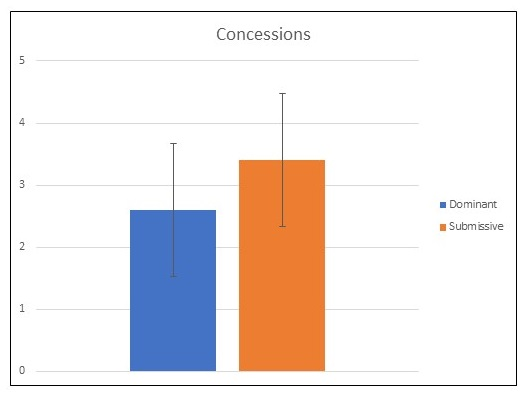
\includegraphics[width=3in]{plots/conced}
			\end{figure}
		
		\par Hypothesis (H3) predicted that agents with higher dominance will take the lead of the negotiation. Our analysis supported this hypothesis. Indeed, participants rated agents with higher dominance to lead the dialogue (M= 4, SD=0.94) more than agents with lower dominance (M= 2.1, SD = 0.88). \emph{p$<$0.01}.(see figure  \ref{lead})
				\begin{figure}[h]
					\centering
					\caption{\label{lead} The results for hypothesis H3}
					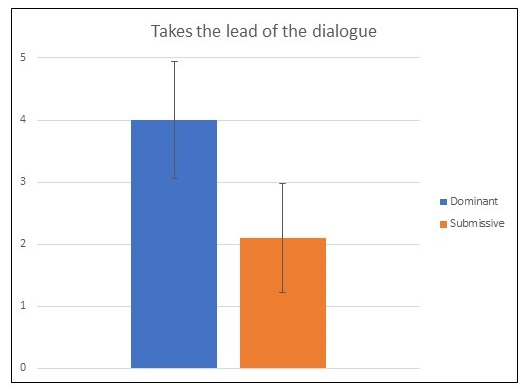
\includegraphics[width=3in]{plots/lead}
				\end{figure}
		\par Our final hypothesis predicted that participants will not perceive a difference in the behaviors of agents initiated with similar preferences. We ran the same experiment by changing the initial preferences of agents to be similar.  Our analysis supported the hypothesis. Indeed, No significant difference in the agents behaviors were perceived by the participants. The results are presented in the table \ref{resume} and figure \ref{fig:H4}.
	\begin{table}
		
	\begin{tabular}{|l|c|c|c|}
	
		\hline
		   & H1 & H2 & H3 \\
		\hline
		Higher dominant agent & (M=3.7, SD=1.17) & (M=3, SD=1.15) &(M=3.88, SD=0.99) \\
		\hline
		Lower dominant agent & (M=3.7, SD=0.82) & (M=3.4, SD=0.7) & (M=2.63, SD=1.19)\\
		\hline
		p-value &  \emph{p $>$ 0.1}  & \emph{p $>$ 0.1}  & \emph{p = 0.1} \\
		\hline
	\end{tabular}
		\caption{\label{resume} Analysis of the results for H4}
	\end{table}
	
		\begin{figure}[!htb]
			\minipage{0.32\textwidth}
			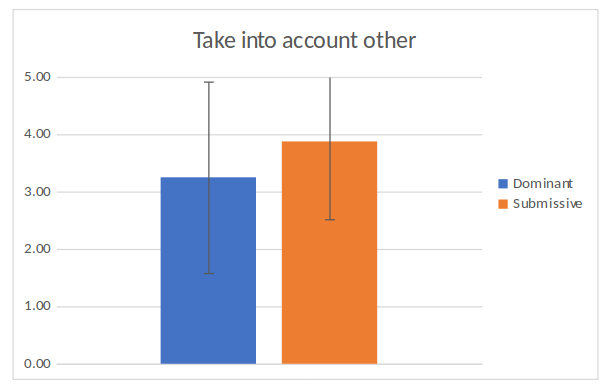
\includegraphics[width=\linewidth]{plots/H4/other.png}
			\caption{Results for H1}\label{fig:other}
			\endminipage\hfill
			\minipage{0.32\textwidth}
			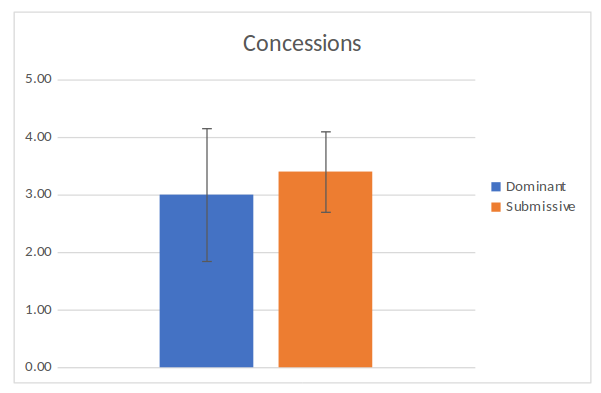
\includegraphics[width=\linewidth]{plots/H4/concession.png}
			\caption{Results for H2}\label{fig:concede}
			\endminipage\hfill
			\minipage{0.32\textwidth}%
			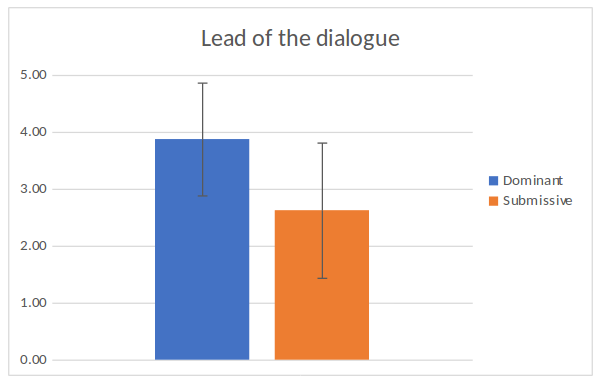
\includegraphics[width=\linewidth]{plots/H4/lead.png}
			\caption{Results for H3}\label{fig:lead}
			\endminipage
			
			\caption{\label{fig:H4} The results of analysis for the similar preferences condition}
		\end{figure}
				
	 \subsection{Discussion}
	 \par  The results from our experiment provided good support to the claim that the relation of dominance affect agent's behaviors in negotiation situations. We found that people perceive this difference in the agent's behaviors depending on the relation of dominance.  Indeed, three of our four hypotheses were confirmed. We predicted that dominant with higher dominance will be perceived as more individualist and self centred. Consistent withe this prediction, agents with higher dominance lead the negotiation. However, our second hypothesis was not confirmed by our analysis. Behaviors related to the concessions were not perceived by our participants.  
	 
	 \textit{Limitations} The results presented have a number of limitations. Participants judged the dialogues from an external point which might influence the engagement in the the process of judging agent behavior. The next step, is to experiment our model with an interaction with humans.. 
	 
	 \section{Conclusion and future works}
	% ================== BIBLIO ===============
	\vskip 4pt
	\bibliographystyle{plain}
	\bibliography{Library}
	\end{document}